\documentclass{assignment}

\course{ECO 120-04}
\name{Lucas Reddinger}
\date{Wednesday 30 November 2022}
\doctitle{Assignment 11: The money market}

\begin{document}
\RaggedRight

\beginassignment{}

\emph{Due Monday 5 December.} Please submit hardcopy at the beginning of class (11:00 a.m.), or if you prefer, under the door of Wimberly Hall 339C by 10:50 a.m.

\ornamentalrule

Suppose that due to hyperinflation in Argentina, a massive influx of demand for the U.S.~dollar arises from Argentines.

\begin{enumerate}

\item Using the model of the money market (for the U.S.~dollar), please illustrate how the prevalence of this new demand affects the nominal interest rate and the quantity of money.

\vspace{2.0\baselineskip}

\begin{center}
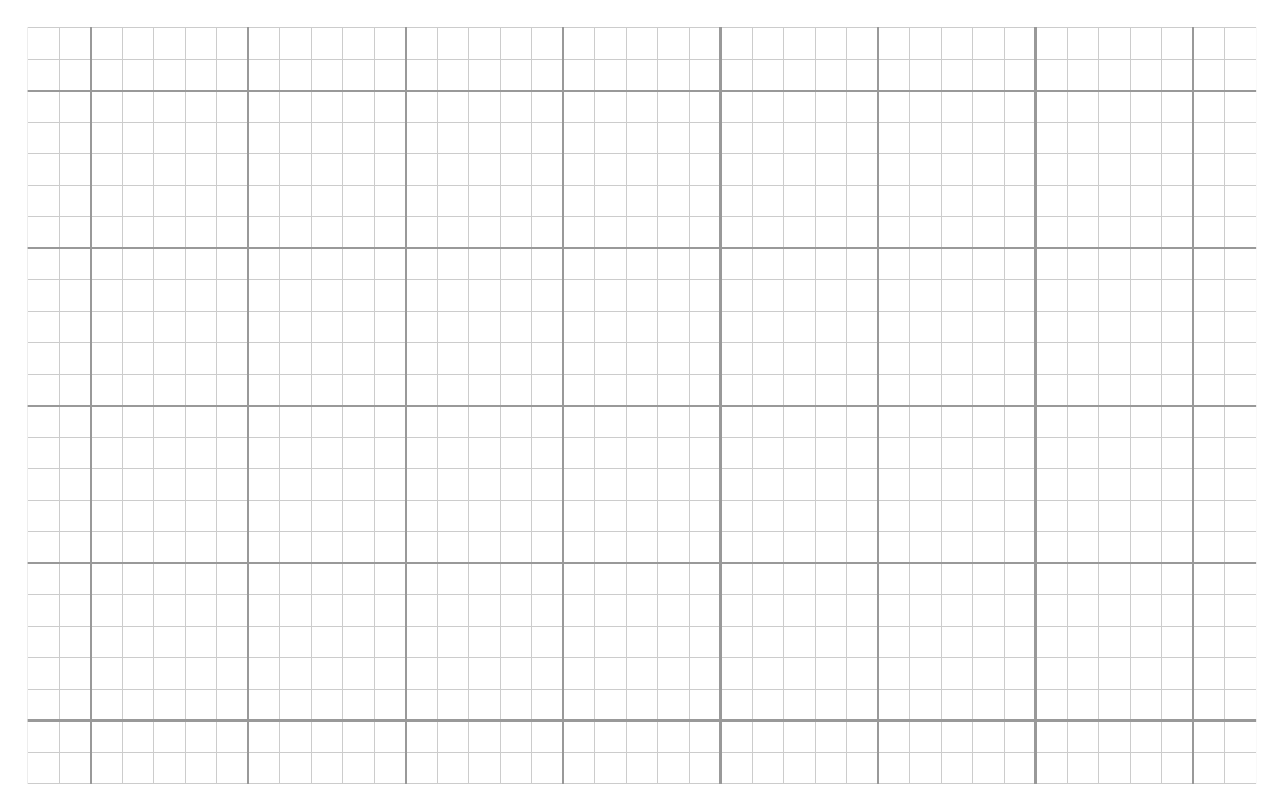
\begin{tikzpicture}[x=4mm, y=4mm]
\clip(3,3) rectangle (42,27);
\draw[step=4mm, very thin, black!20!white] (0,0) grid (60,120);
\draw[step=20mm, thick, black!40!white] (0,0) grid (60,120);
\end{tikzpicture}
\end{center}

\vspace{1.0\baselineskip}

\item Prior to this change in demand for the U.S.~dollar, the macroeconomy was in equilibrium at full employment. Using the model of aggregate demand and aggregate supply, please illustrate and explain the impact of the change in interest rates---from question 1, above---on GDP and the aggregate price level.

\vfill

\begin{center}
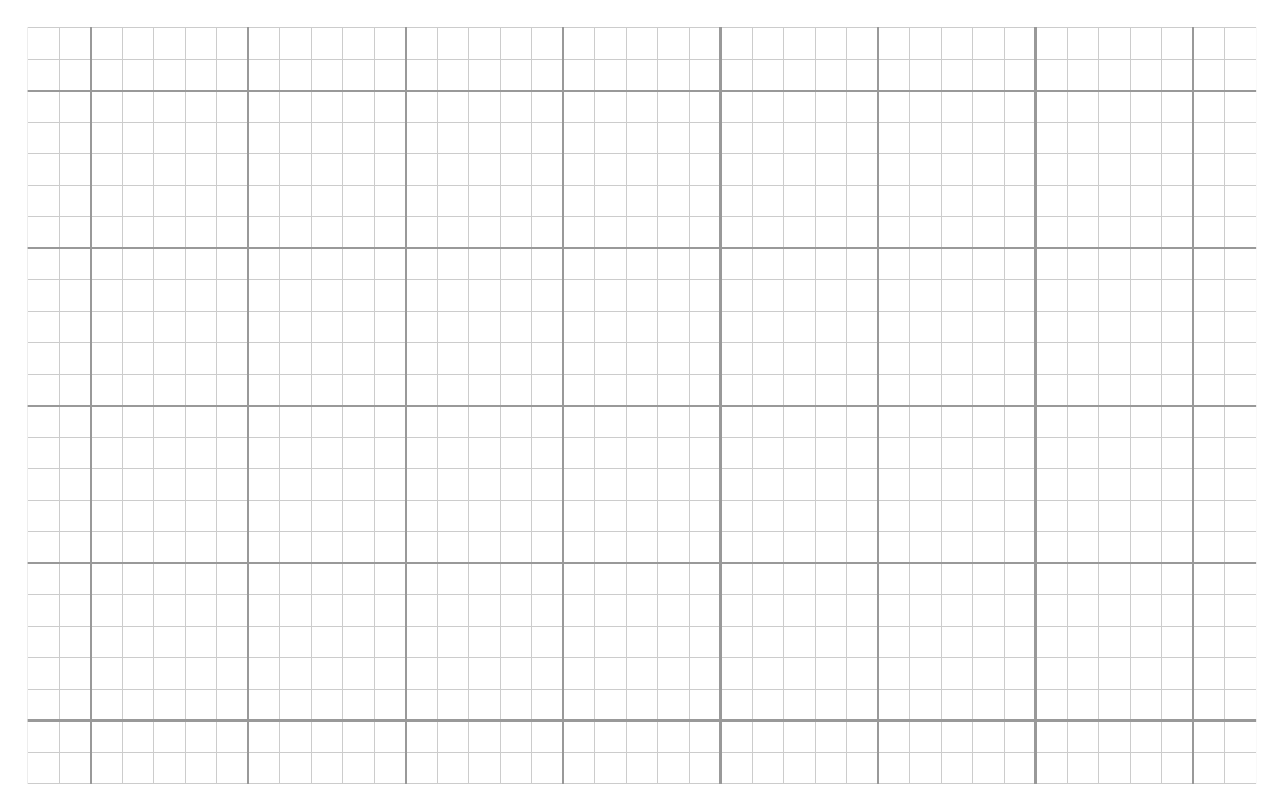
\begin{tikzpicture}[x=4mm, y=4mm]
\clip(3,3) rectangle (42,27);
\draw[step=4mm, very thin, black!20!white] (0,0) grid (60,120);
\draw[step=20mm, thick, black!40!white] (0,0) grid (60,120);
\end{tikzpicture}
\end{center}

\vspace{1.0\baselineskip}

\item The Federal Reserve wants to \emph{exactly} reverse the impact of the change in interest rates on the macroeconomy.  What is one way in which the Fed can do this? Using the model of the money market illustrate the impact of such a policy on the nominal interest rate and the quantity of money.

\vfill

\begin{center}
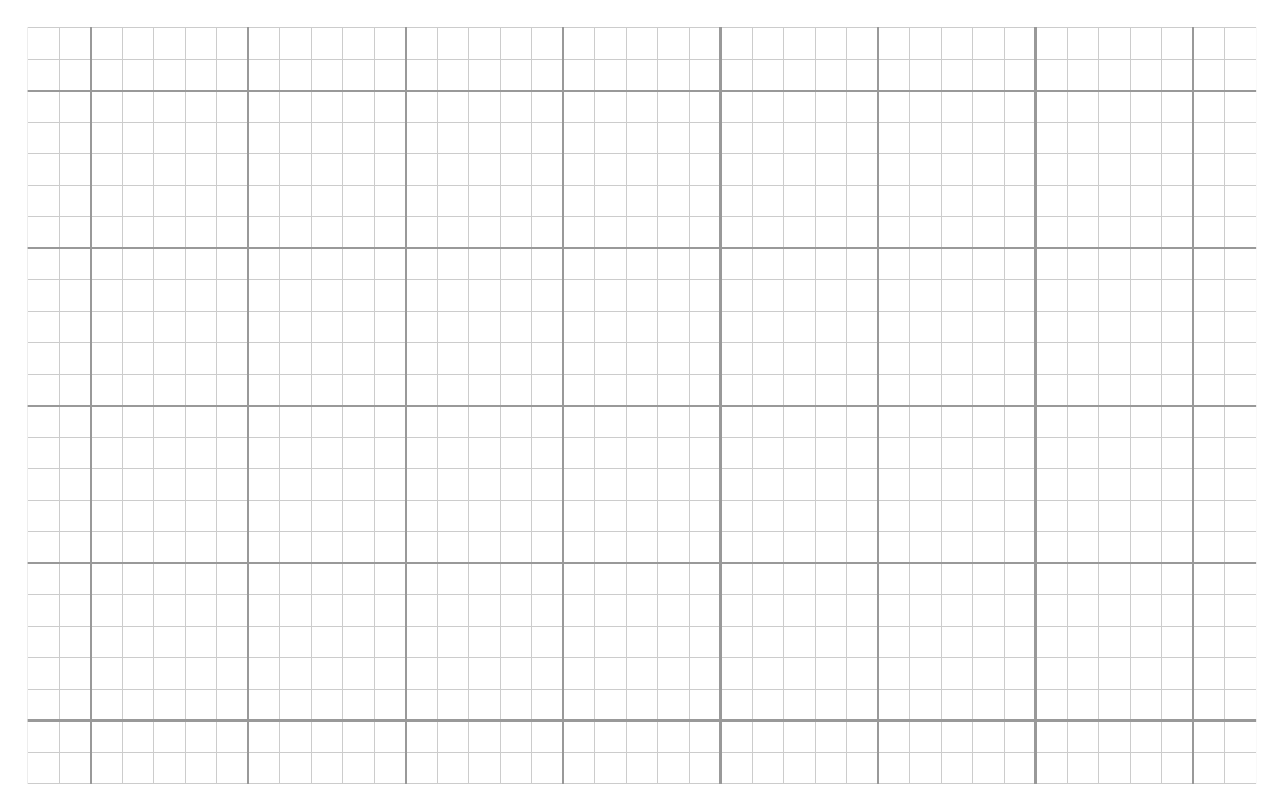
\begin{tikzpicture}[x=4mm, y=4mm]
\clip(3,3) rectangle (42,27);
\draw[step=4mm, very thin, black!20!white] (0,0) grid (60,120);
\draw[step=20mm, thick, black!40!white] (0,0) grid (60,120);
\end{tikzpicture}
\end{center}

\end{enumerate}

\end{document}
